\documentclass[12pt, a4paper]{article}
\usepackage[francais]{babel}
\usepackage{caption}
\usepackage{graphicx}
\usepackage[T1]{fontenc}
\usepackage{listings}
\usepackage{geometry}
\usepackage{array,multirow,makecell}
\usepackage{float}
\usepackage[colorlinks=true,linkcolor=black,anchorcolor=black,citecolor=black,filecolor=black,menucolor=black,runcolor=black,urlcolor=black]{hyperref}
\setcellgapes{1pt}
\makegapedcells
\usepackage{fancyhdr}
\pagestyle{fancy}
\lhead{}
\rhead{}
\chead{}
\rfoot{\thepage}
\lfoot{Baumgaertner - Karapetyan}
\cfoot{}
\renewcommand{\footrulewidth}{0.4pt}
\renewcommand{\headrulewidth}{0.4pt}

% \usepackage{mathpazo} --> Police à utiliser lors de rapports plus sérieux

\begin{document}
\begin{titlepage}
	\newcommand{\HRule}{\rule{\linewidth}{0.5mm}} 
	\center 
	\textsc{\LARGE iut de colmar}\\[6.5cm] 
	\textsc{\Large R4.ROM.10}\\[0.5cm] 
	\textsc{\large Opérateurs de télécoms}\\[0.5cm]
	\HRule\\[0.75cm]
	{\huge\bfseries Rapport final MPLS-TE}\\[0.4cm]
	\HRule\\[1.5cm]


	% Utiliser les lignes qui suivent dans le cas où il y a plusieurs membres
	%------------------------------------
	\begin{minipage}{0.4\textwidth}
		\begin{flushleft}
			\large
			\textit{RT222}\\
			Martin \textsc{Baumgaertner}
		\end{flushleft}
	\end{minipage}
	~
	\begin{minipage}{0.4\textwidth}
		\begin{flushright}
			\large
			\textit{RT222}\\
			Mikhaïl \textsc{Karapetyan}
		\end{flushright}
	\end{minipage}
    
	%------------------------------------
    %------------------------------------
	% \textsc{\large martin baumgaertner}\\[0.5cm] % S'il y que moi qui écrit
    %------------------------------------
	\vfill\vfill\vfill
	{\large\today} 
	\vfill
\end{titlepage}
\newpage
\tableofcontents
\newpage



\newpage
\section{Introduction}

\section{Préparation et réservation des ressources}
\subsection{Question 1}
Le résultat de la commande \textbf{show mpls traffic-eng topology}, nous voyons bien 
l'ensemble des liens qui font partis de la topologie MPLS. 

\begin{figure}[h]
    \centering
    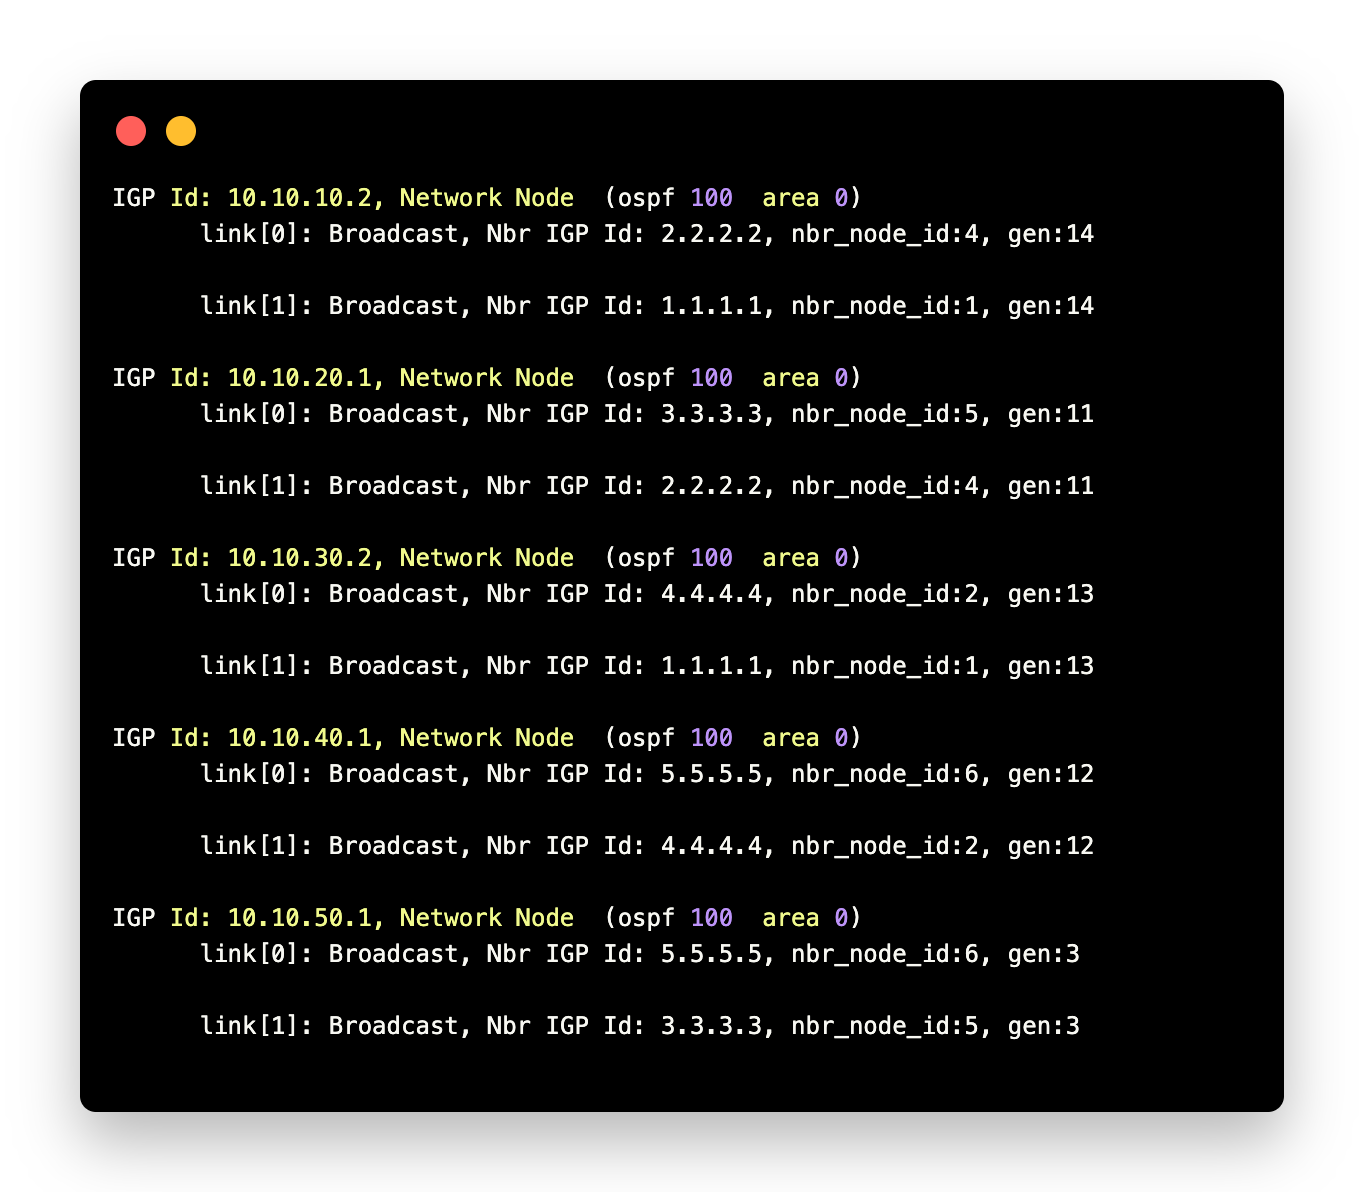
\includegraphics[width=1\textwidth]{img/code1.png}
    \caption{Topologie MPLS}
    \label{fig:script1}
\end{figure}
\newpage
Pour chaque lien nous avons un récaputulatif de l'ensemble des informations des liens.
Voici un exemple pour le lien \textbf{1.1.1.1}
\begin{figure}[h]
    \centering
    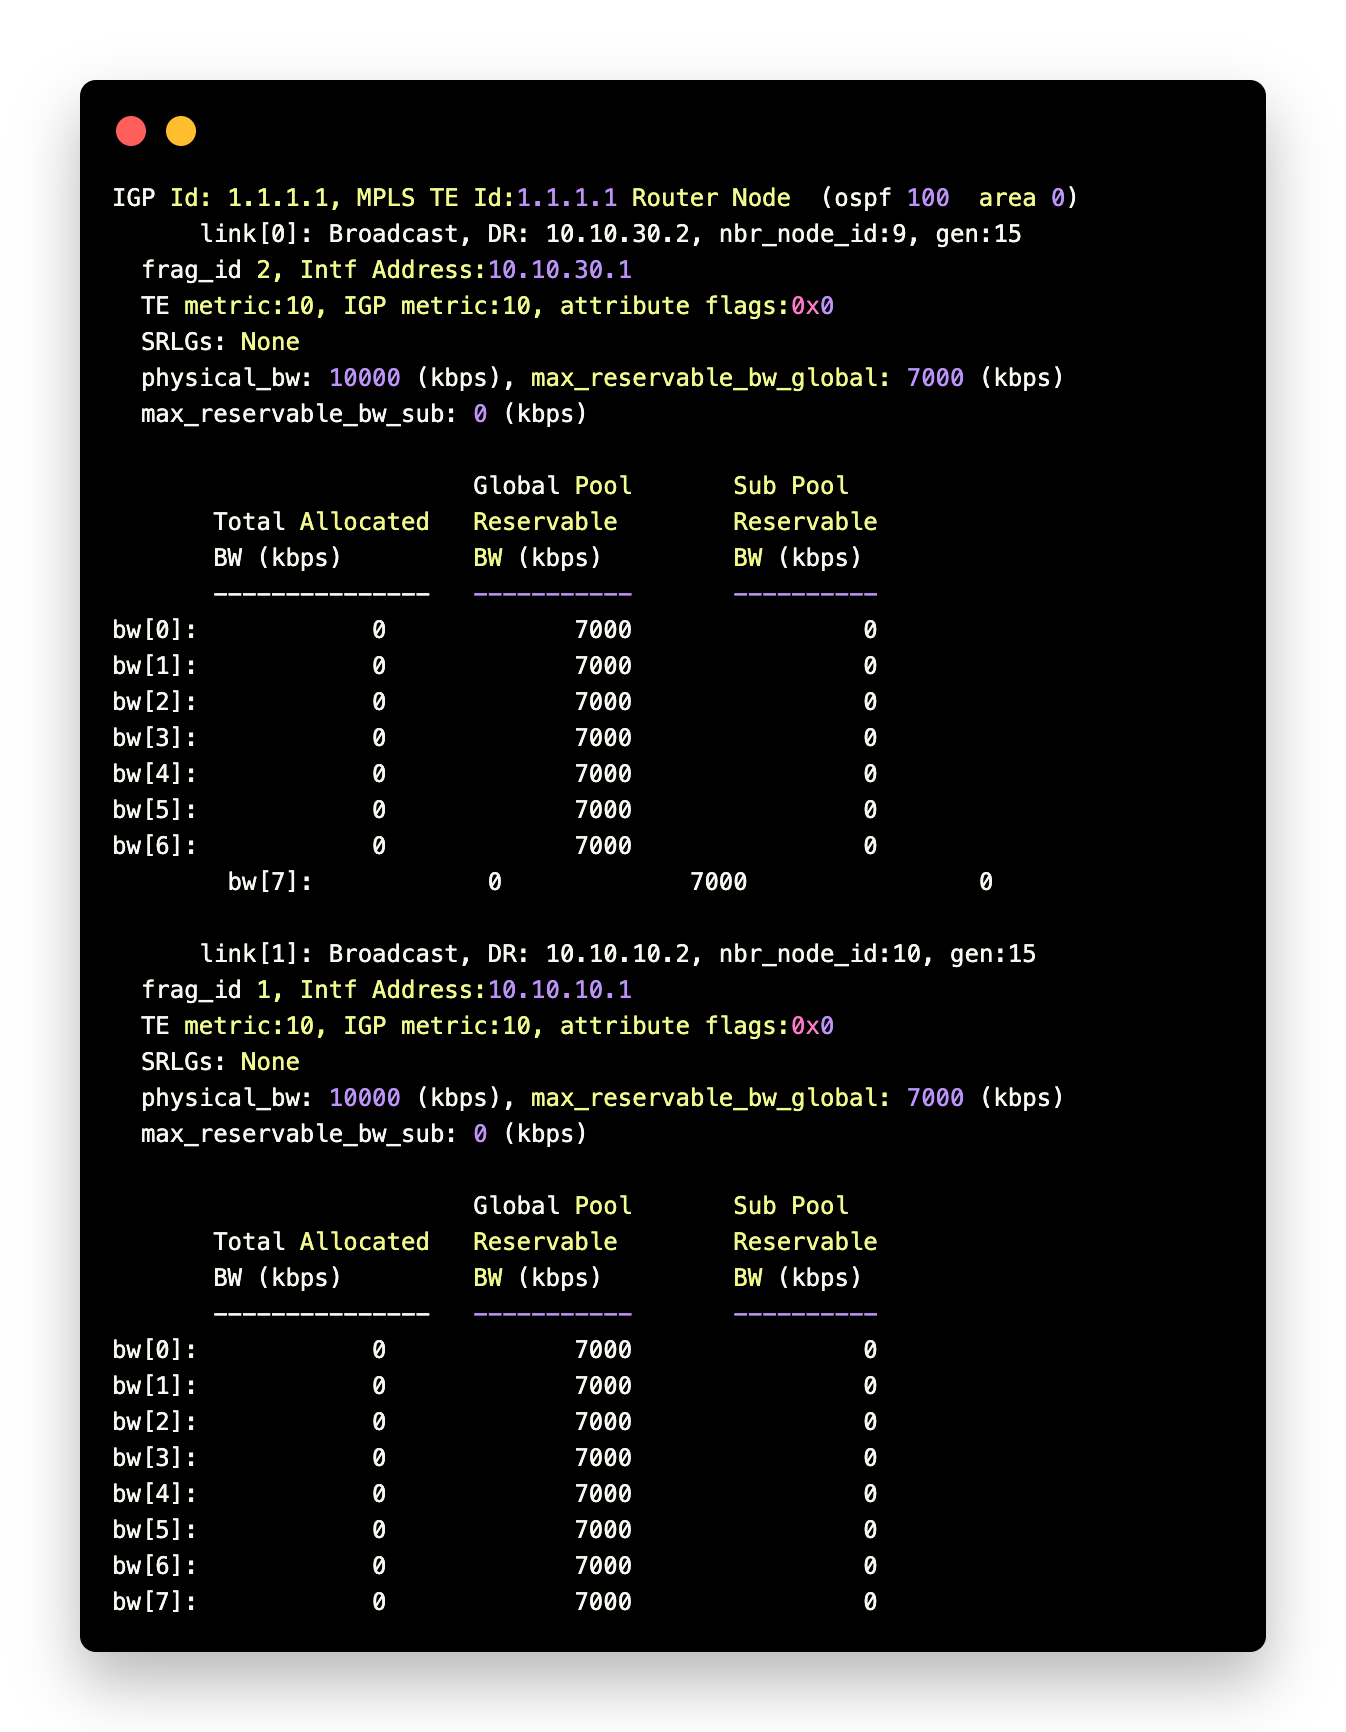
\includegraphics[width=0.8\textwidth]{img/code2.png}
    \caption{Informations des liens}
    \label{fig:script2}
\end{figure}

\subsection{Question 2}
La capacité des liens physiques en termes de bande passante est de 10 000kbps. Nous 
pouvons retrouver cette valeur lors de la commande précédente. \textbf{physical\_bw : 10000 (kbps)}

\subsection{Question 3}
La valeur de la métrique IGP et TE est de 10. Nous pouvons retrouver cette valeur lors de la première commande : \textbf{igp\_metric : 10} et \textbf{te\_metric : 10}


\section{Configuration du tunnel MPLS-TE}
\subsection{Configuration de l’entête du tunnel}
\subsubsection{Question 1}
Voici donc la configuration du Tunnel0
\begin{figure}[h]
    \centering
    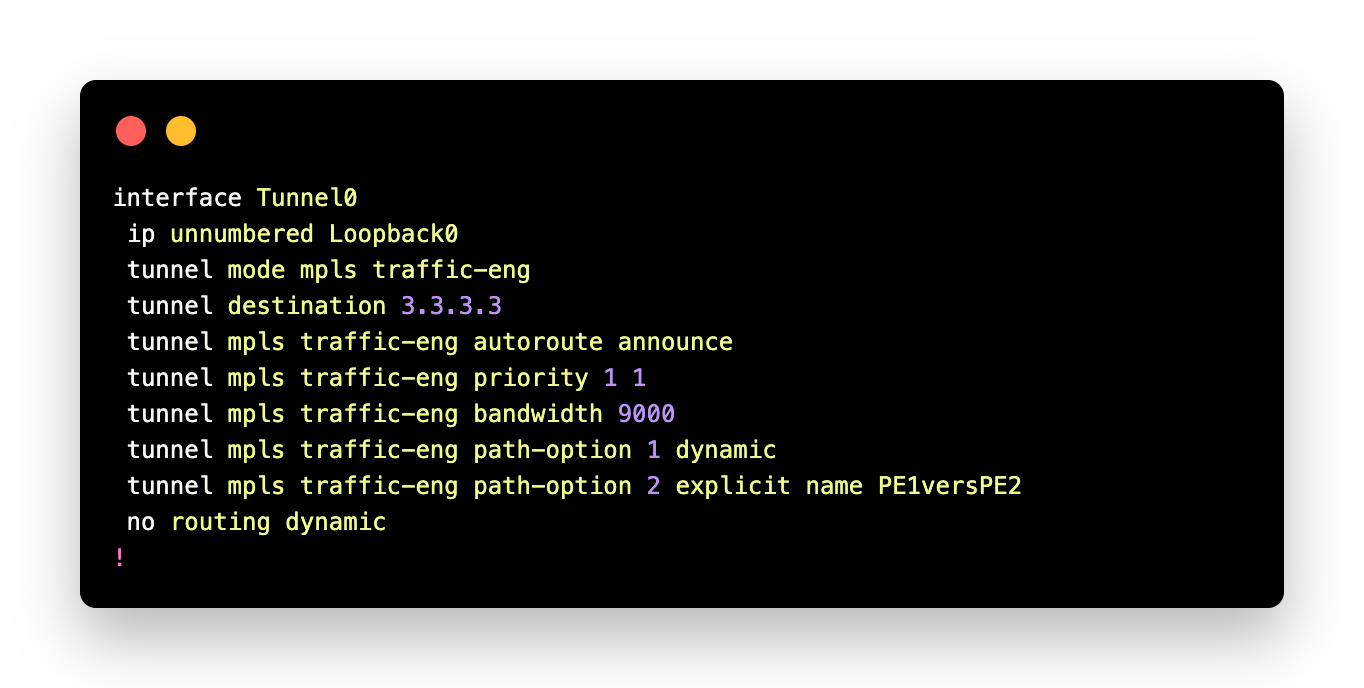
\includegraphics[width=1\textwidth]{img/code3.png}
    \caption{Configuration du Tunnel0}
    \label{fig:script3}
\end{figure}

\newpage
\subsubsection{Question 2}
Pour vérifier la table de commutation nous devons faire la commande ci-après. Nous 
aurons comme la résultat donc la table de commutation du tunnel0.
\begin{figure}[h]
    \centering
    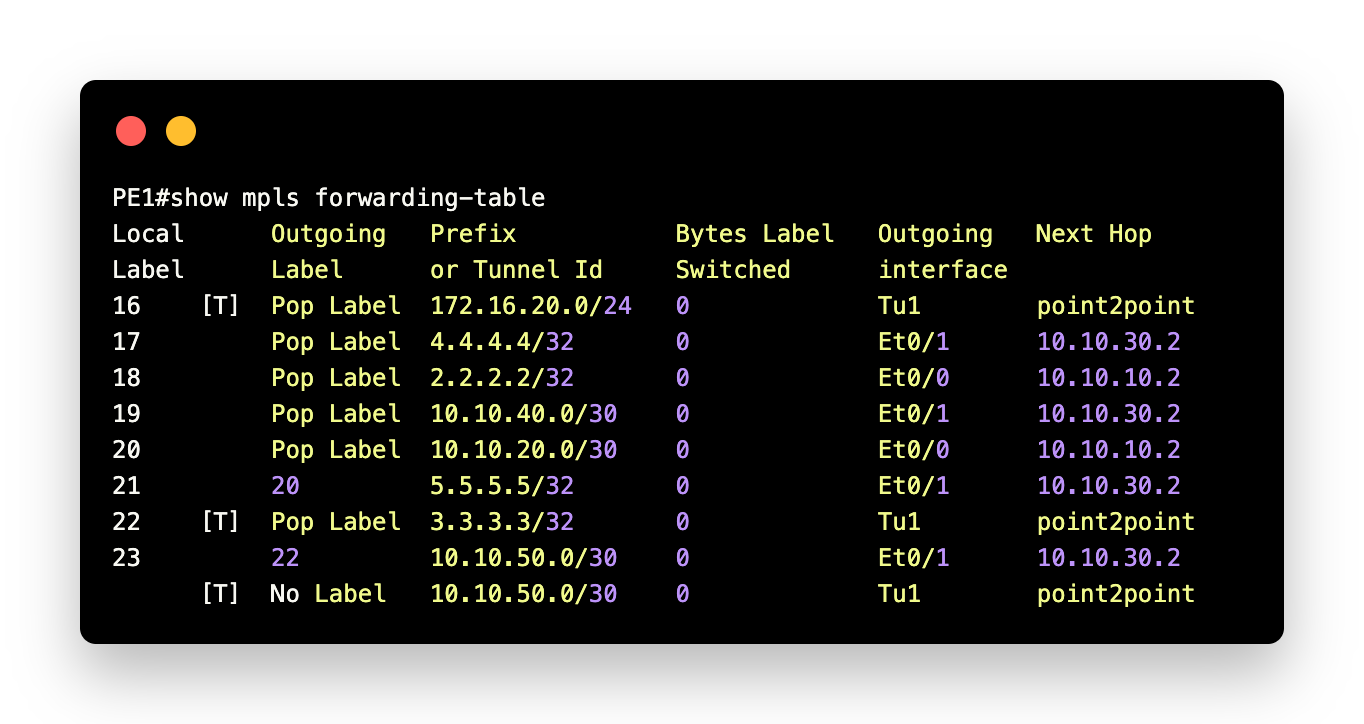
\includegraphics[width=1\textwidth]{img/code4.png}
    \caption{Table de commutation du tunnel0}
    \label{fig:script4}
\end{figure}

\newpage
\subsubsection{Question 3}
Pour afficher la table de routage du PE1 et voir combien d’entrées utilisent le tunnel
il faut faire la commande suivante. 

\begin{figure}[h]
    \centering
    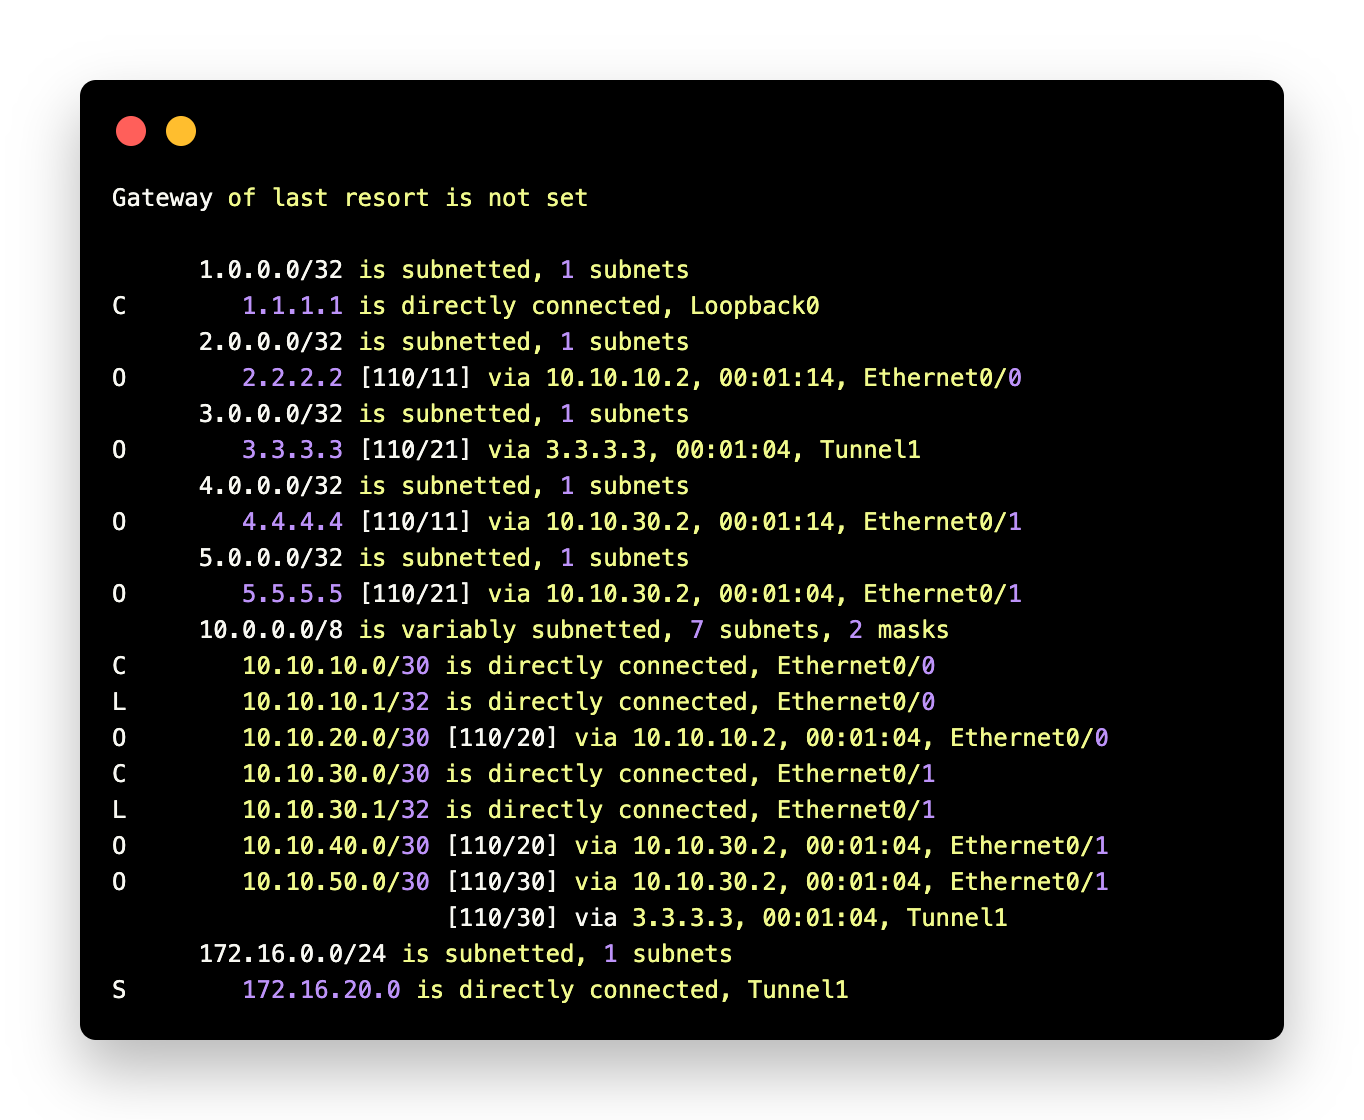
\includegraphics[width=1\textwidth]{img/code5.png}
    \caption{Table de routage du PE1}
    \label{fig:script5}
\end{figure}
\newpage

\subsubsection{Question 4}
Voici ce que nous donne la commande \textbf{show mpls traffic-eng tunnels} sur le PE1.
Le chemin utilisé par le tunnel est donc \textbf{Explicit Route: 10.10.10.2 10.10.20.2 10.10.20.1 3.3.3.3}

\begin{figure}[h]
    \centering
    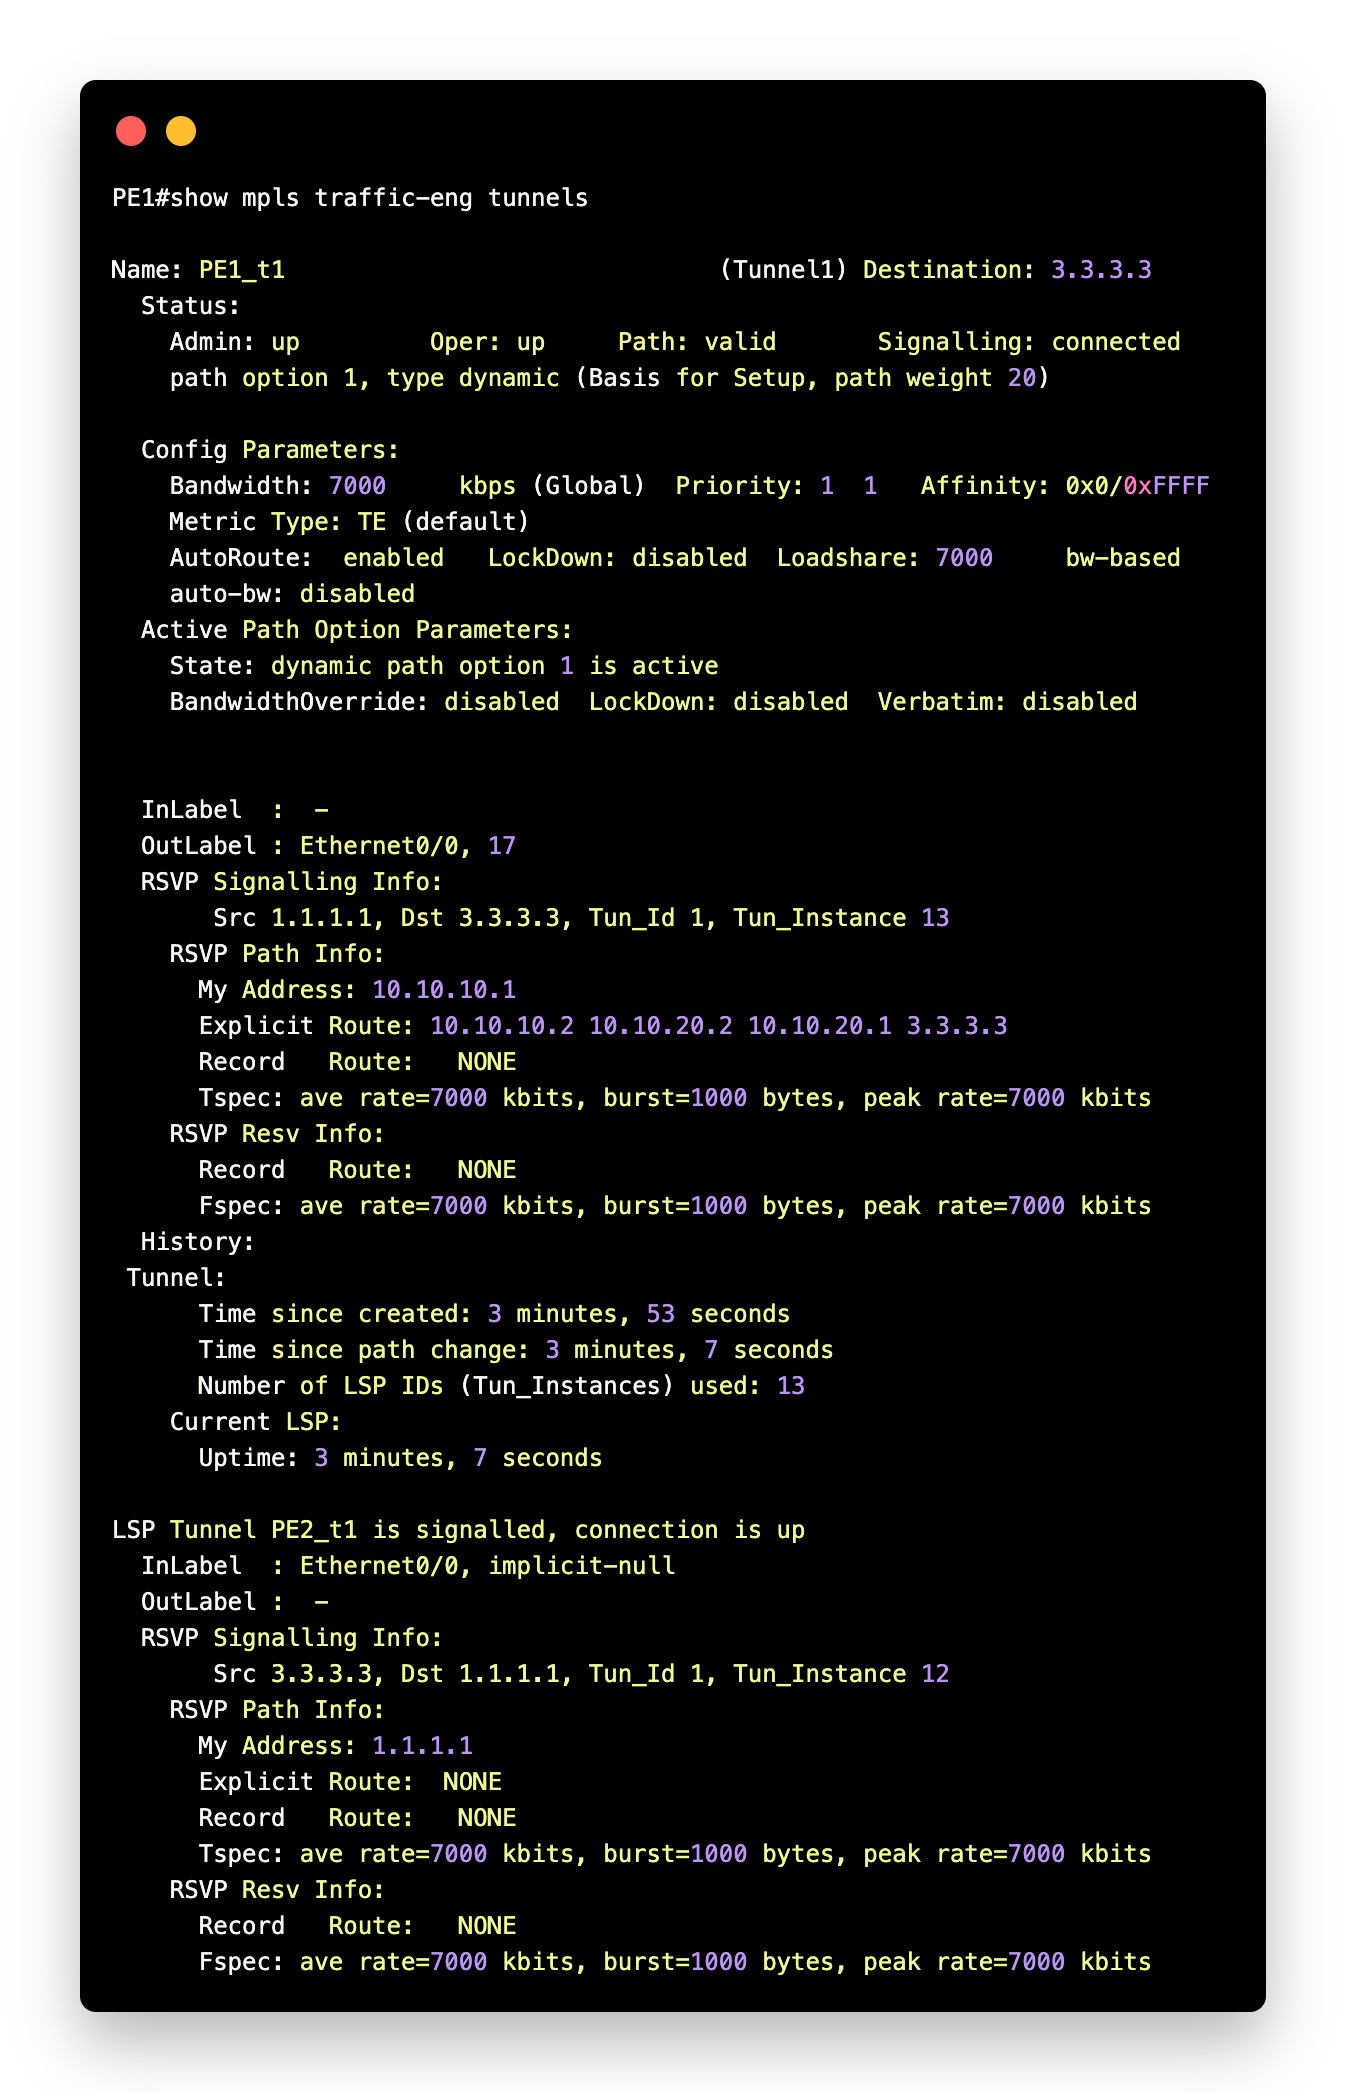
\includegraphics[width=0.66\textwidth]{img/code6.png}
    \caption{Chemin utilisé par le tunnel}
    \label{fig:script6}
\end{figure}

\newpage
\subsubsection{Question 5}
Les valeurs sont donc correct, nous pouvons voir ci-après que tout 
correspond bien  à 7000kbps, ce qui avait été initialement configuré.
\begin{figure}[h]
    \centering
    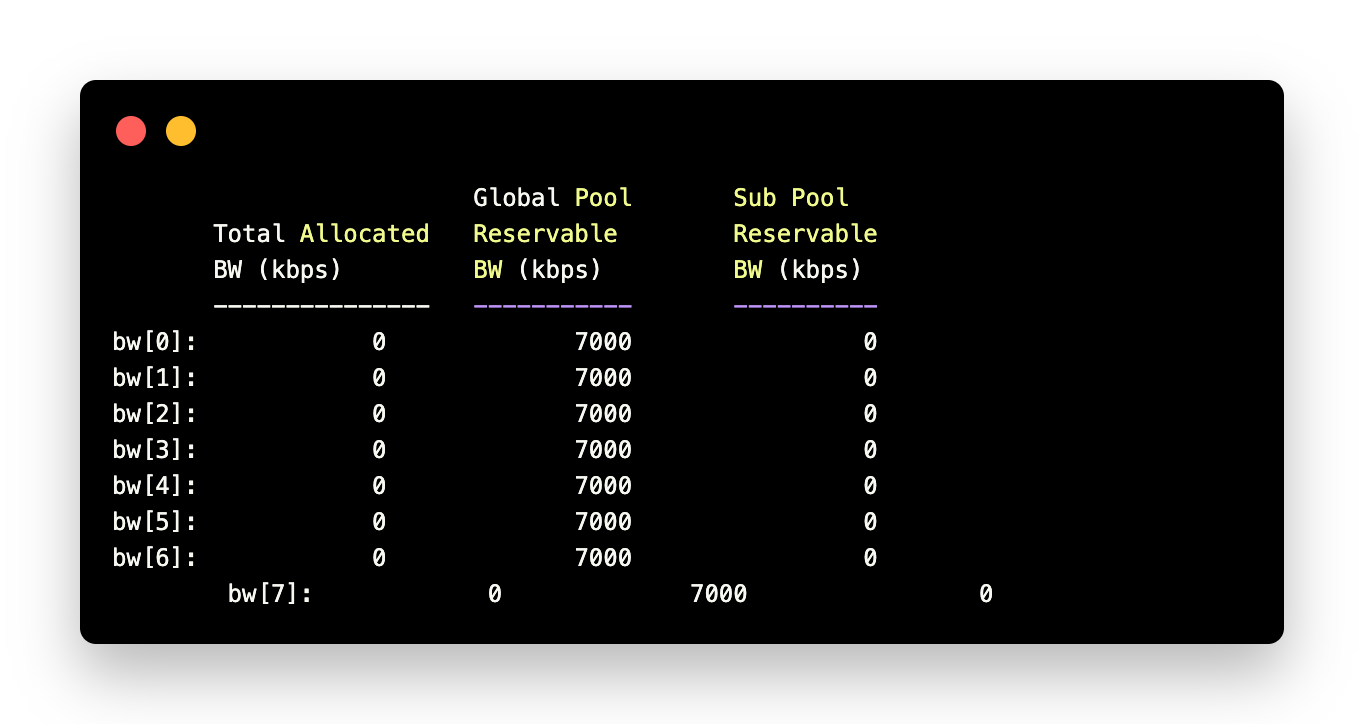
\includegraphics[width=1\textwidth]{img/code7.png}
    \caption{Valeurs de la bande passante}
    \label{fig:script7}
\end{figure}

\subsubsection{Question 6}
C'est tout à fait normal car nous n'avons pas encore monté les liens dans les
deux sens, car P2 c'est un routeur intémédiaire, et il fait juste passer les 
paquets du tunnel. Nous n'observerons jamais de traffic MPLS sur les 
routeurs intémédiaires. 

\newpage
\subsubsection{Question 7}
Lorsque nous faisons un traceroute depuis PE1 vers 3.3.3.3 nous obtenons 
ce résultat : 
\begin{figure}[h]
    \centering
    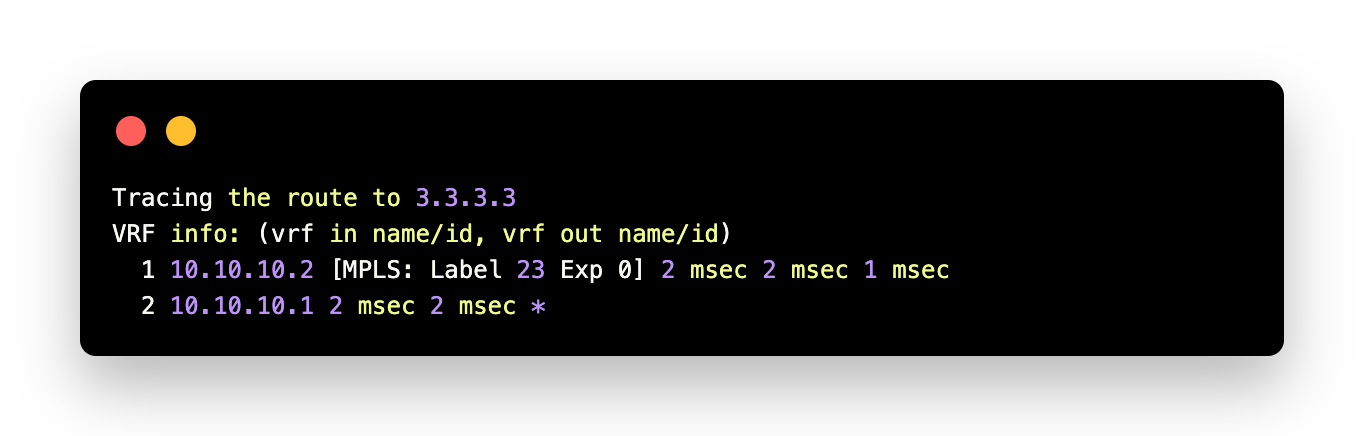
\includegraphics[width=0.7\textwidth]{img/code8.png}
    \caption{Traceroute depuis PE1}
    \label{fig:script8}
\end{figure}

Nous remarquons que le label utilisé pour le premier saut vient de la table
de commutation de MPLS c'est le local label 23 qui correspond.\\

Ci-après, on voit bien que le label 23 est utilisé dans le paramètre InLabel du 
routeur PE1. Nous voyons bien que sur le PE2 le InLabel est différent. 
\begin{figure}[h]
    \centering
    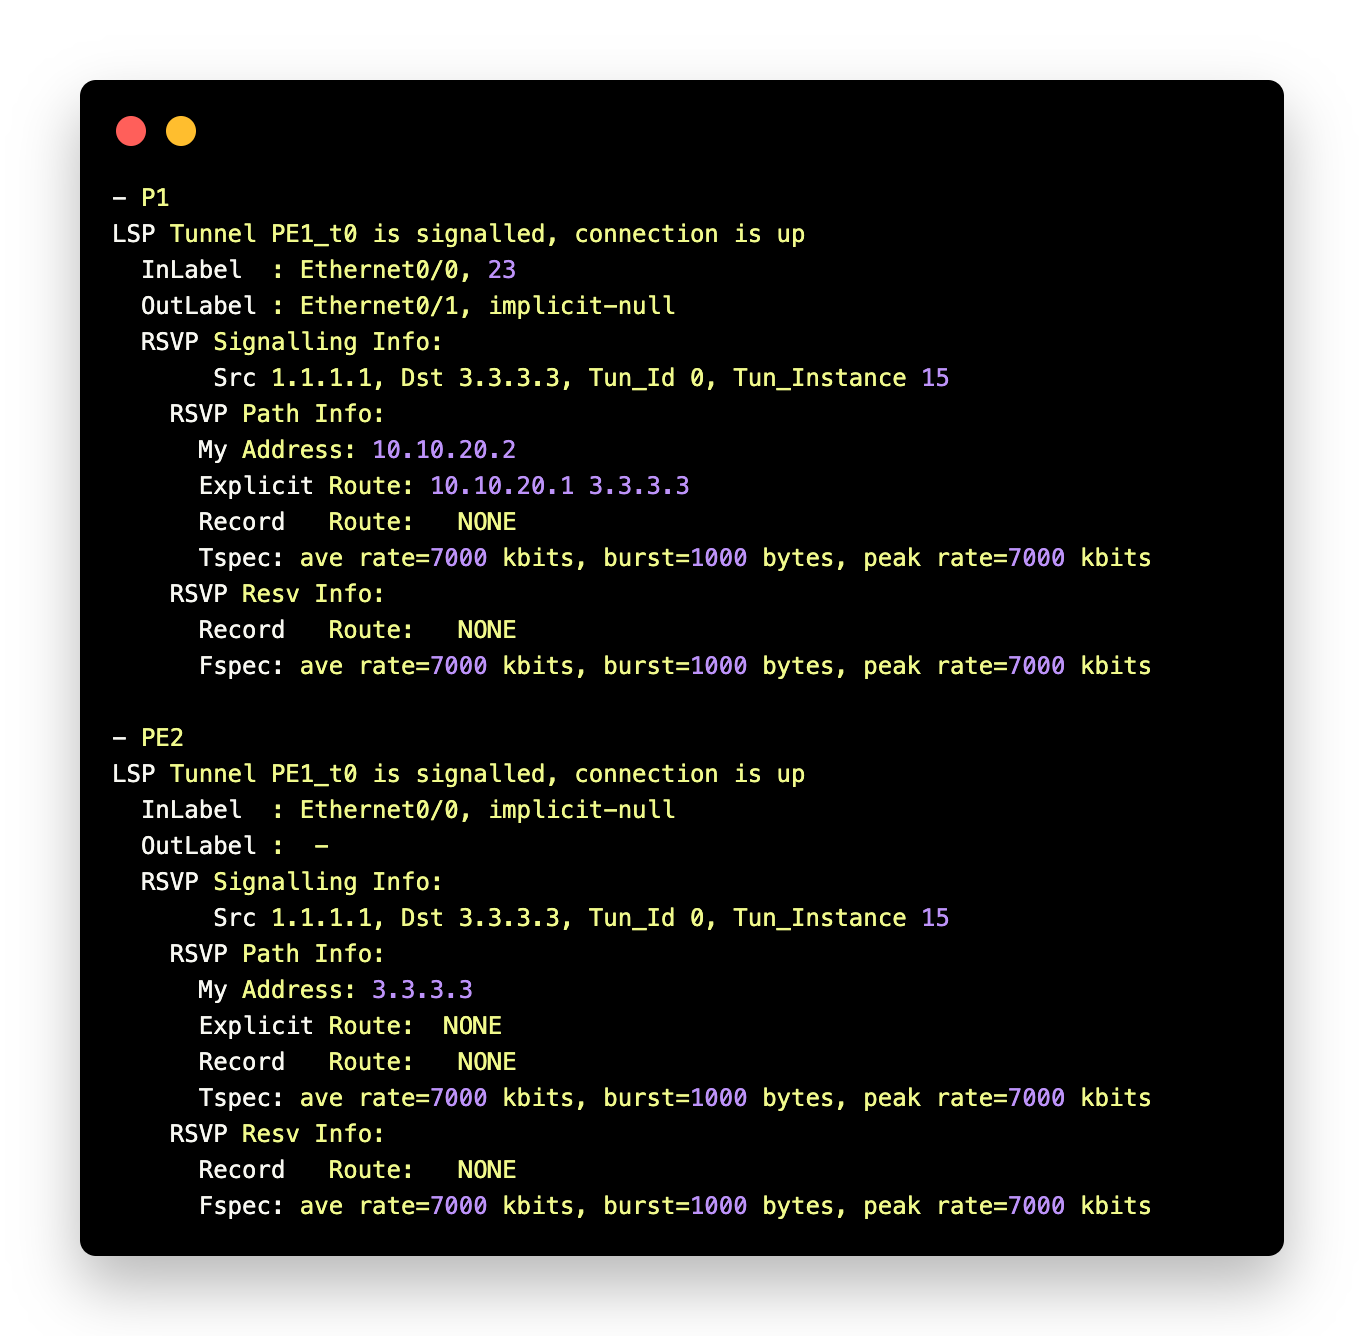
\includegraphics[width=0.6\textwidth]{img/code9.png}
    \caption{Show MPLS traffic-eng tunnels}
    \label{fig:script9}
\end{figure}

\newpage
\subsubsection{Question 8}
\begin{figure}[h]
    \centering
    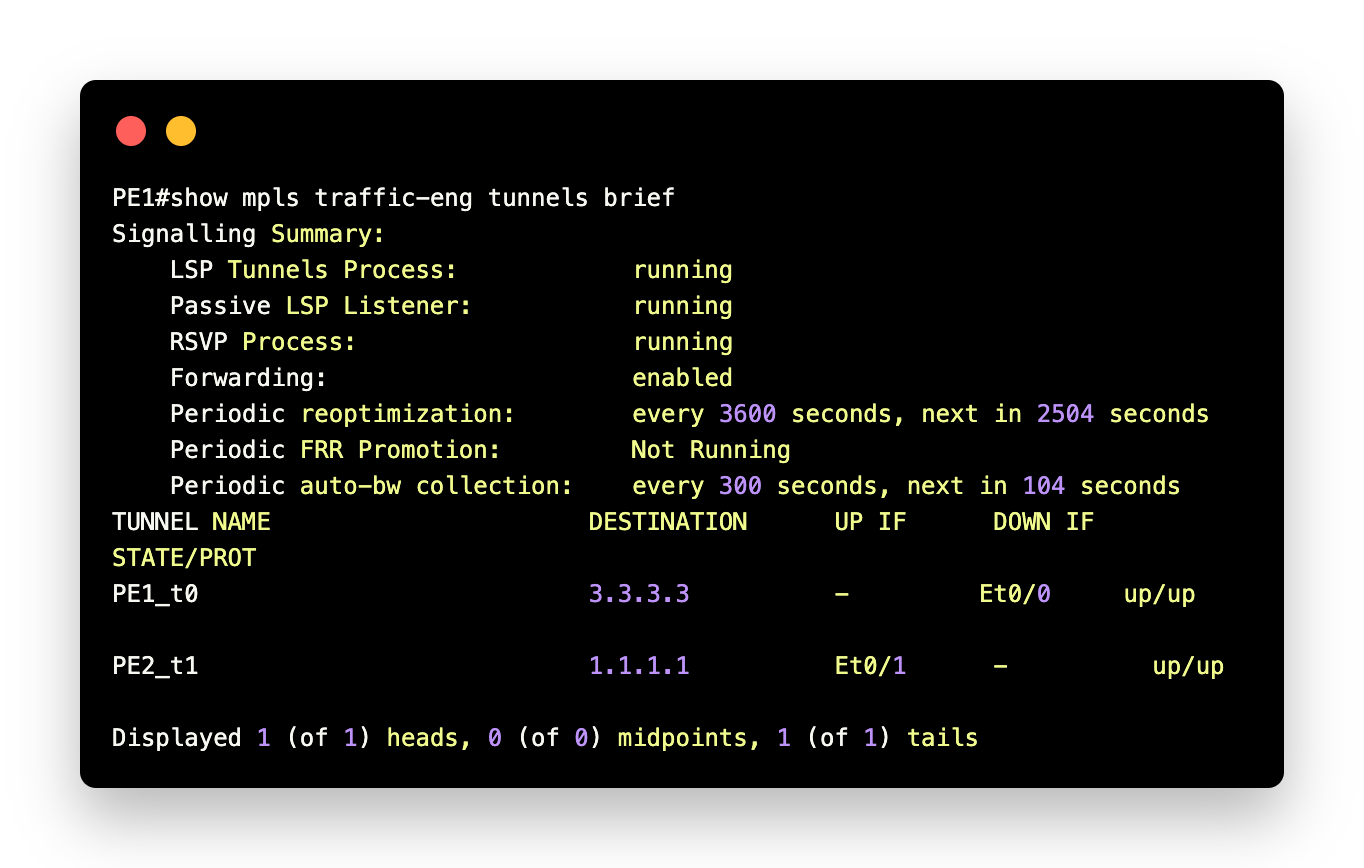
\includegraphics[width=1\textwidth]{img/code10.png}
    \caption{Show mpls traffic-eng tunnels brief}
    \label{fig:script10}
\end{figure}

La commande "show mpls traffic-eng tunnels brief" affiche une liste succincte 
des tunnels d'ingénierie de trafic MPLS configurés sur un périphérique réseau.
Cette commande fournit les informations suivantes :\\
\begin{itemize}
    \item Tunnel Name: Le nom du tunnel MPLS Traffic Engineering.
    \item State: L'état du tunnel (UP ou DOWN).
    \item Destination: L'adresse de destination du tunnel.
\end{itemize}

\newpage
\subsection{Communication entre les deux clients avec MPLS-TE}
\subsubsection{Question 1}
Pour vérifier la connexion avec le client CE2 depuis le réseau local
du CE1 en effectuant un ping étendu il faut faire la commande suivante :\\

\textbf{CE1\#ping}\\

Le ping ne fonctionne pas car pour l'instant nous avons un seul tunnet dans un seul
sens donc les deux côtés ne peuvent pas encore commuiqué. Car quand on ping depuis 
CE1 le paquet s'envoie mais le retour ne peut pas se faire car le paquet se perd. 

% \subsubsection{Question 2}


% \subsubsection{Question 3}


% \subsubsection{Question 4}


% \subsubsection{Question 5}


% \subsubsection{Question 6 a)}


% \subsubsection{Question 6 b)}

\subsection{MPLS-TE avec chemin explicite}
\subsubsection{Question 1}
\begin{figure}[h]
    \centering
    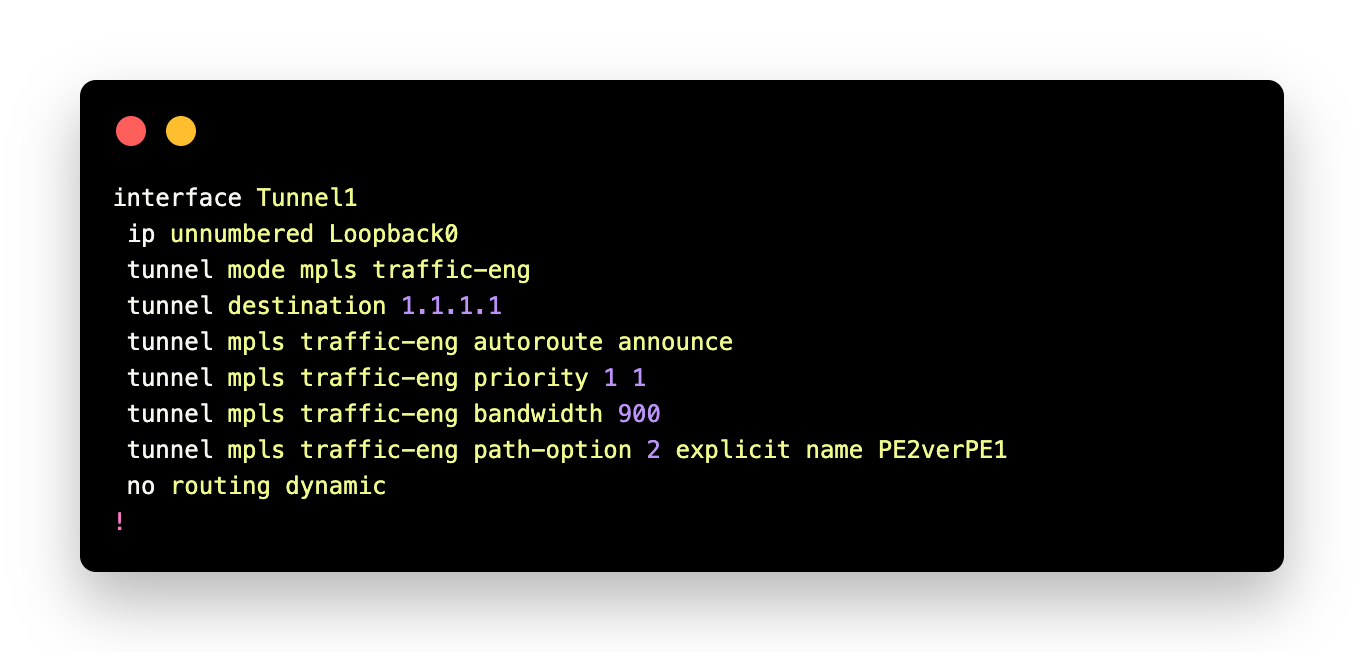
\includegraphics[width=1\textwidth]{img/code11.png}
    \caption{Déclaration du Tunnel1}
    \label{fig:script11}
\end{figure}
Voici donc ci-dessus la déclaration du Tunnel1.

\newpage
\subsubsection{Question 2}
Voici la commande pour déclarer le chemin explicite en utilisant l’option ‘strict’ :\\
\textbf{tunnel mpls traffic-eng path-option 2 explicit name PE2verPE1\\}
\textbf{ip explicit-path name PE2verPE1 enable\\
next-address 5.5.5.5\\
next-address 4.4.4.4\\
next-address 1.1.1.1\\}

\subsubsection{Question 3}
Voici donc la commande pour orienter tout trafic à destination du réseau 172.16.10.0/24 vers le tunnel que nous
venons de créer.
\textbf{ip route 172.16.10.0 255.255.255.0 Tunnel1}

\subsubsection{Question 4}
J'éffectue donc la commande \textbf{show mpls traffic-eng tunnels brief}
et je peux constater donc que tout fonctionne normalement comme le démontre
la figure ci-dessous.
\begin{figure}[h]
    \centering
    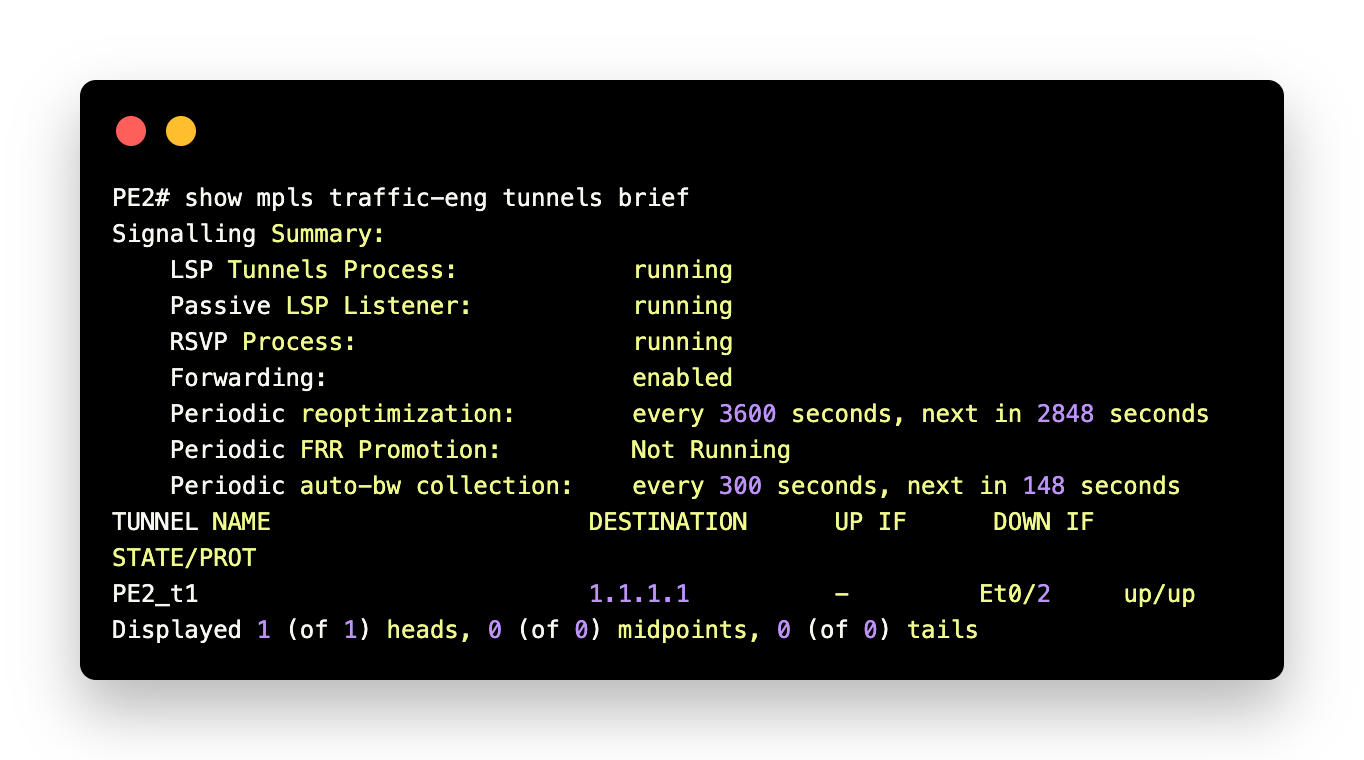
\includegraphics[width=1\textwidth]{img/code12.png}
    \caption{Vériricationn de l'établissement du tunnel}
    \label{fig:script12}
\end{figure}


\subsubsection{Question 5}
Je vérifie à nouveau le ping et nous nous rendons compte que le ping 
fonctionne bien. 
\begin{figure}[h]
    \centering
    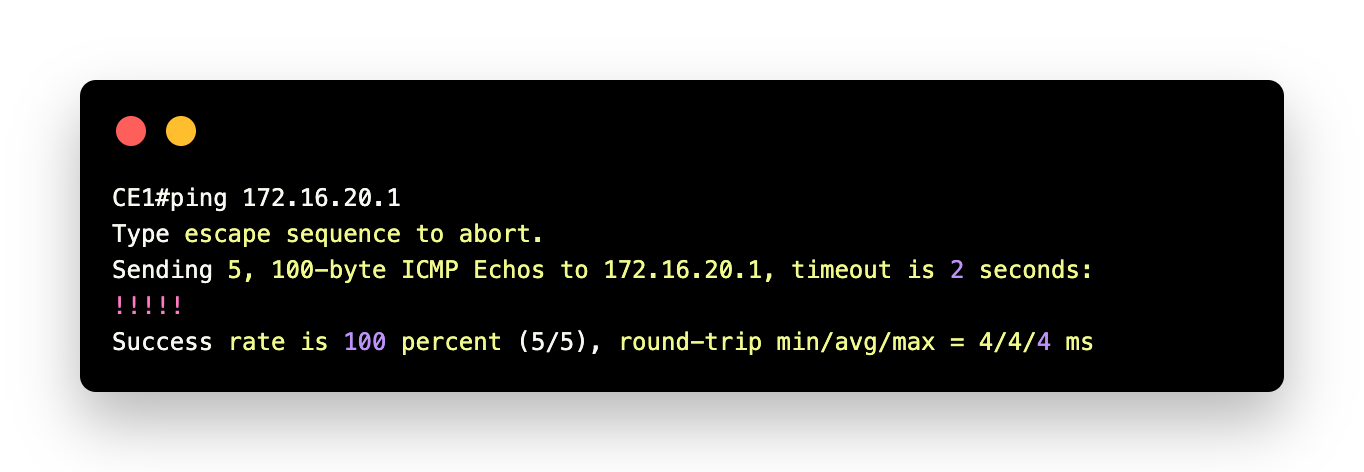
\includegraphics[width=1\textwidth]{img/code13.png}
    \caption{Vériricationn de l'établissement du tunnel}
    \label{fig:script13}
\end{figure}

\subsubsection{Question 6}
J'effectue donc un traceroute sur CE1 et CE2 pour aller respectivement aux deux réseaux locaux
et voici ce que j'obtiens. 



\subsection{Chemin ne satisfaisant pas les contraintes TE.}
\subsubsection{Question 1}
Depuis que nous avons changé la bande passante initialement prévu les pings entre
le CE2 et le CE1 ne fonctionne plus. Cela est dû au fait que la bande passante
passante physique maximale autorisé des interfaces est plus petite que celle atribuée au tunnel.


\newpage
\subsubsection{Question 2}
Voici donc ce que l'on obtient lorsque l'on vérifie la présence d'un chemin qui vérifie certaines contraintes.
\begin{figure}[h]
    \centering
    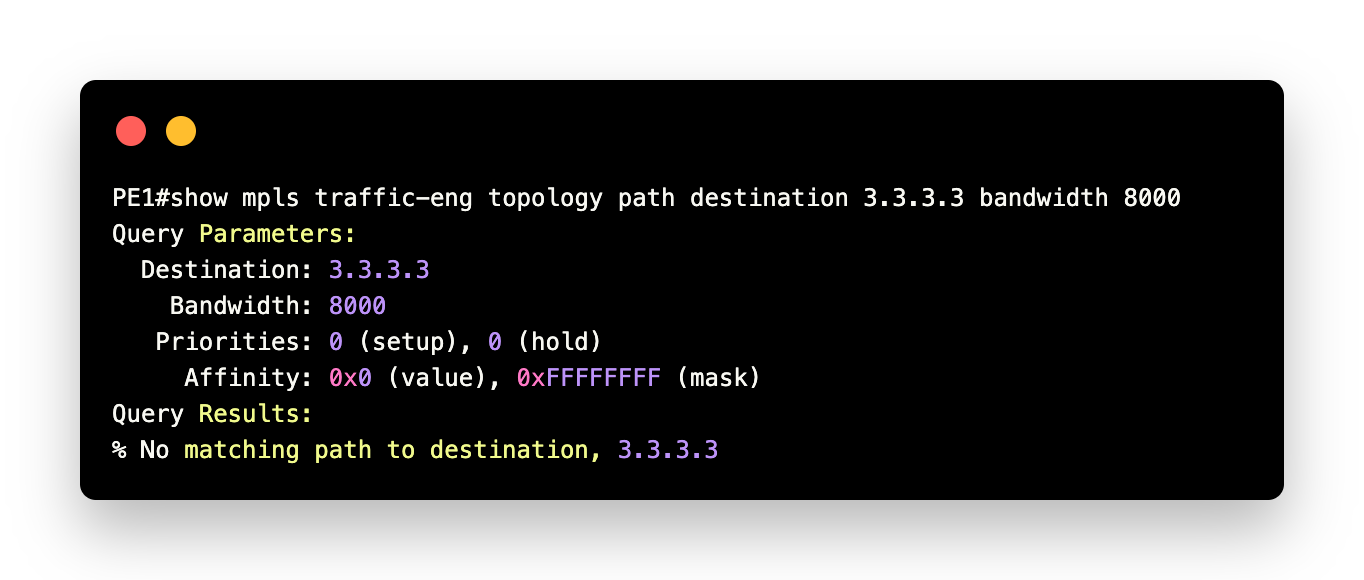
\includegraphics[width=1\textwidth]{img/code14.png}
    \caption{Vériricationn de la présence d'un chemin}
    \label{fig:script14}
\end{figure}

\end{document}